\documentclass[a4paper,14pt]{extreport}
\usepackage[left=1.5cm,right=1.5cm,
    top=1.5cm,bottom=2cm,bindingoffset=0cm]{geometry}
\usepackage[T1,T2A]{fontenc}
\usepackage[utf8]{inputenc}
\usepackage[english,russian]{babel}
\usepackage{amsmath,amsthm,amssymb}
\usepackage{mathtext}
\usepackage{xcolor}
\usepackage{hyperref}
\usepackage{geometry}

\usepackage{fancyhdr, graphicx}

\definecolor{ggreen}{rgb}{0.4,1,0}
\definecolor{rred}{rgb}{1,0.1,0.1}
\definecolor{amber}{rgb}{1.0, 0.75, 0.0}
\definecolor{babyblue}{rgb}{0.54, 0.81, 0.94}
\definecolor{asparagus}{rgb}{0.53, 0.66, 0.42}
\definecolor{chartreuse}{rgb}{0.5, 1.0, 0.0}
\definecolor{darkorchid}{rgb}{0.6, 0.2, 0.8}

\usepackage{tcolorbox}
\usepackage{tikz}
\usepackage[framemethod=TikZ]{mdframed}
\usepackage{wrapfig,boxedminipage,lipsum}
\mdfdefinestyle{MyFrame}{%
linecolor=asparagus,outerlinewidth=2pt,roundcorner=10pt,innertopmargin=\baselineskip,innerbottommargin=\baselineskip,innerrightmargin=20pt,innerleftmargin=20pt,backgroundcolor=gray!10!white}





\begin{document}
\begin{center}
Лищенко Богдан ДП-82 \\
вар. №53
\end{center}



      \begin{enumerate}
\item Якi основнi домiшки, використовують для створення шарiв з акцепторною провiднiстю?\\

Матеріали, що складаються з елементів IV групи таблиці Менделєєва, акцепторами елементів Кремнію та Германію є елементи III, тобто це Бор, Індій, Алюміній, Титан, Галій.\\

\item Накресліть еквівалентну схему інтегрального біполярного п-р-п транзистора.

\begin{figure}[h]
\center{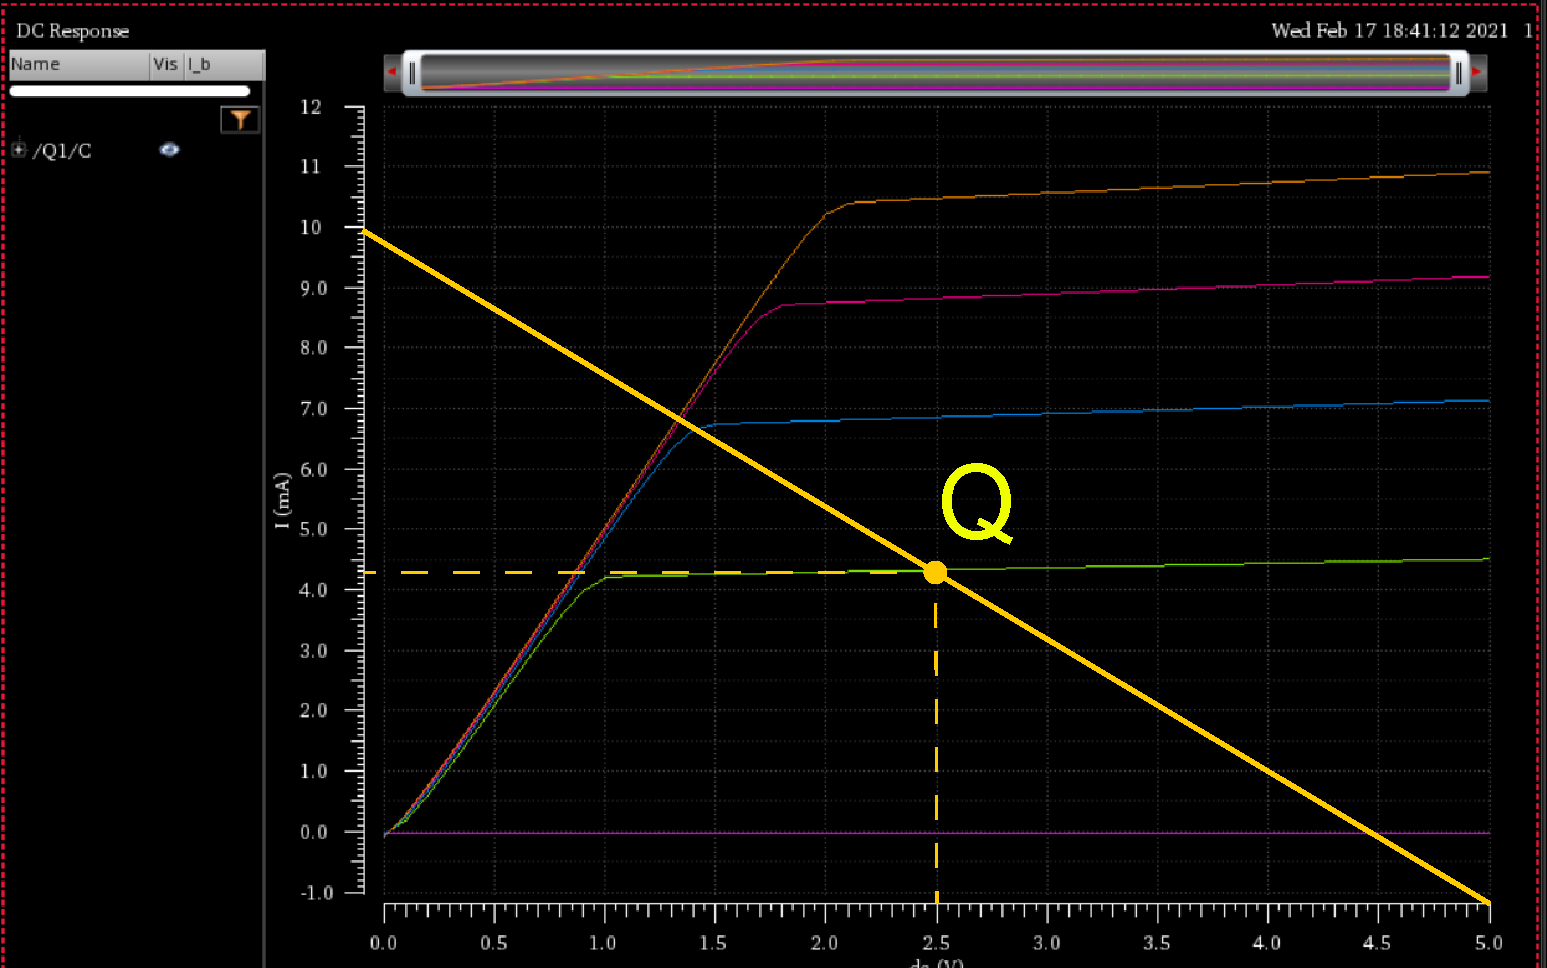
\includegraphics[width=0.5\linewidth]{1.png}}
\end{figure}
\item Емітер\\

\item Накресліть поперечний розріз епітаксіального планарного біполярного транзистора з ізоляцією р – п переходом .\par
\begin{figure}[h!]
\center{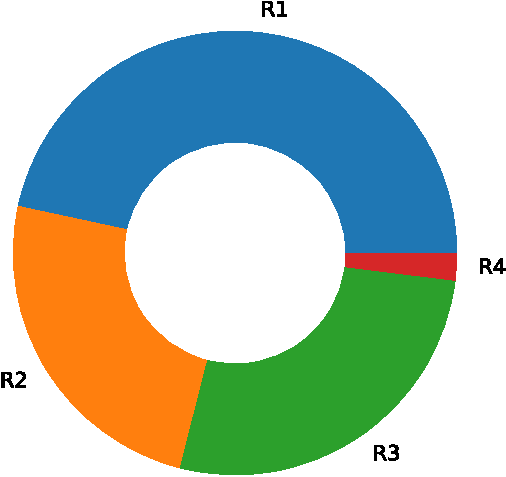
\includegraphics[width=0.4\linewidth]{2.png}}
\end{figure}
\newpage
\begin{figure}[h!]
\item  Показати п’ять можливих схем діодного включення біполярного транзистора.\par
\center{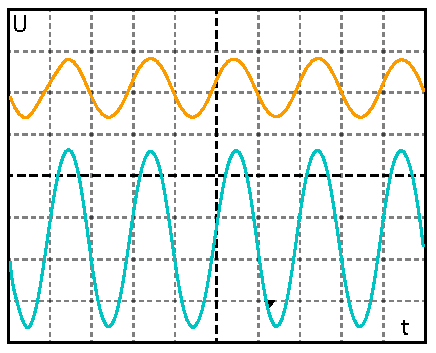
\includegraphics[width=0.8\linewidth]{4.png}}
\end{figure}

\item Для чого використовують в планарно – епітаксіальних біполярних n-p-n транзисторах ІС прихований $n^+$ шар?\\

Для зменшення об'ємного опору області колектора\\


\item  Який тип транзисторів в інтегральних схемах є основним — n-p-n чи p-n-p тип, і чому?\\

n-p-n тому що р–n–р-транзистори, виготовляють водночас з n–р–n-транзисторами у тих шарах напівпровідникової структури, які створюються для n–р–n транзистора.\\


\item Визначити коефіцієнти підсилення по струму в схемі із загальною базою, коли значення коефіцієнти підсилення по струму в схемі із із загальним емітером дорівнює 170.\\

$\alpha = \dfrac{170}{1+170} = $ 0,99415204678362573099415204678363\\
\newpage

\item Накресліть розподіл концентрацій домішок в структурі інтегрального планарно - епітаксіального біполярного п-р-п транзистора.\par


\begin{figure}[h!]
\center{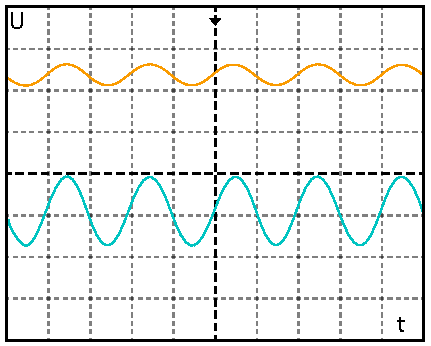
\includegraphics[width=0.3\linewidth]{12.png}}
\end{figure}


\item  Представити вихідні характеристики в схемі з загальним емітером для біполярних транзисторів в ІС з прихованим n + шаром та без прихованого
n + шару.\par

\begin{figure}[h!]
\center{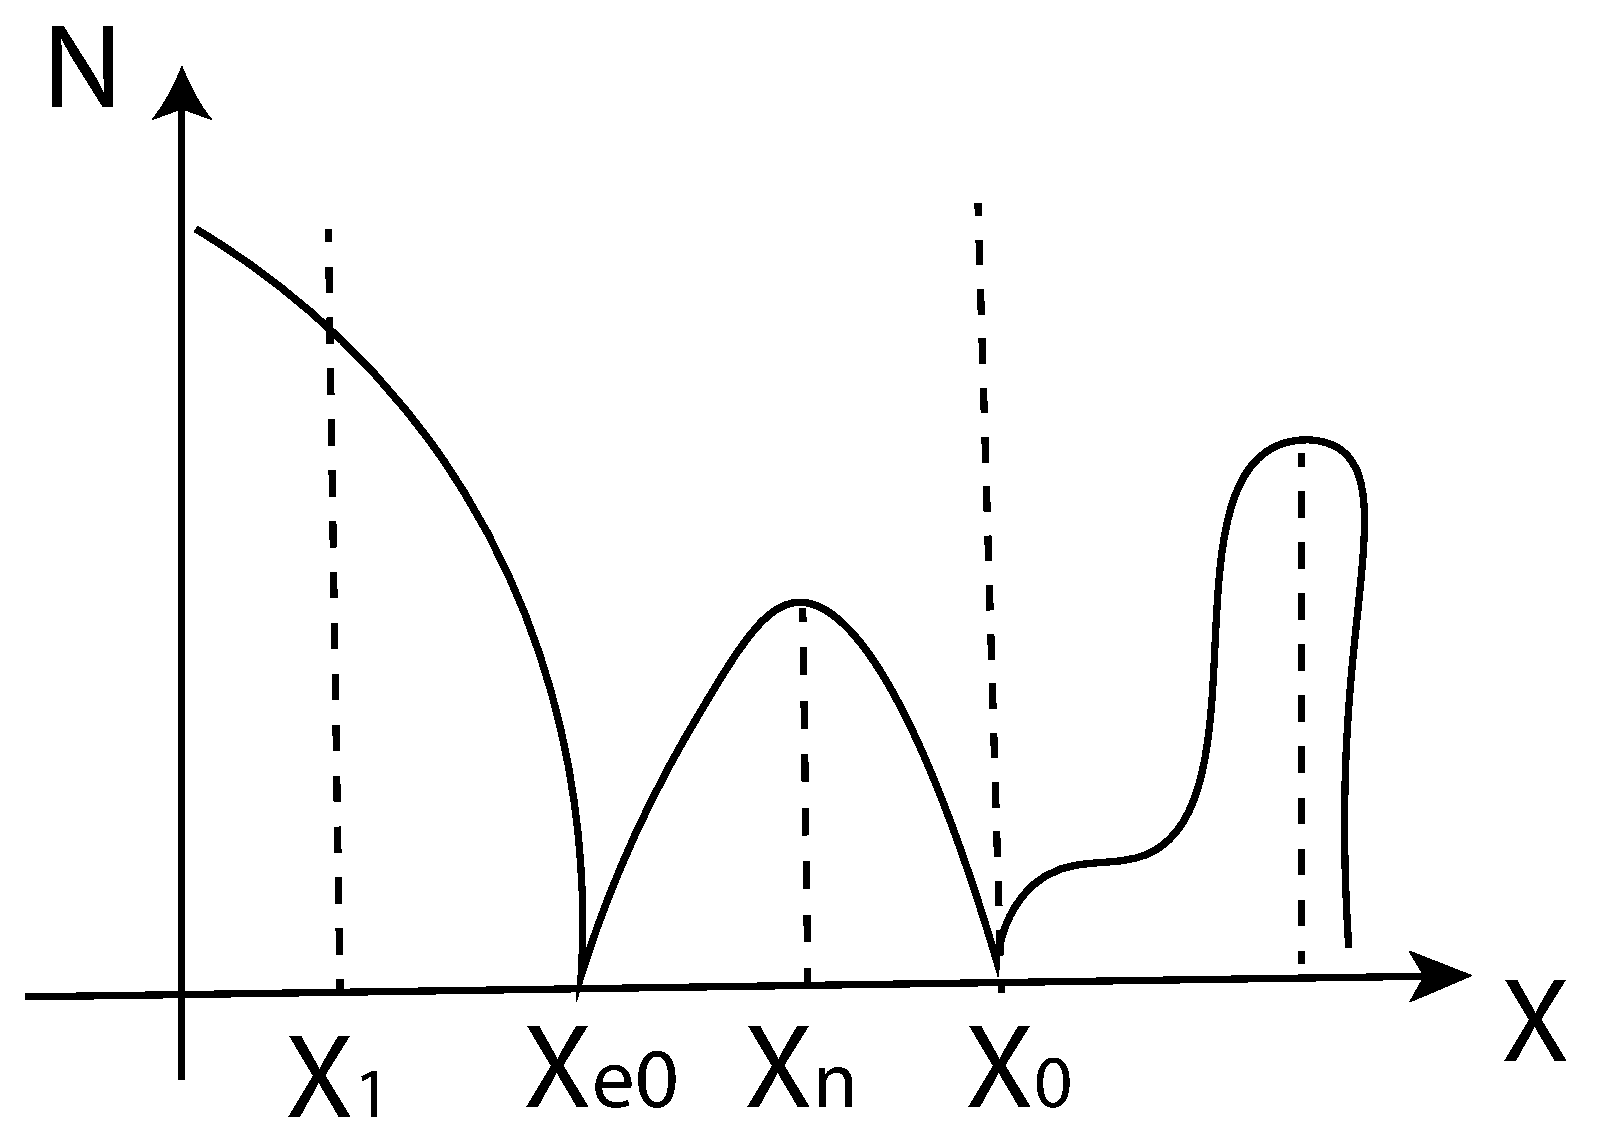
\includegraphics[width=0.3\linewidth]{3.pdf}}
\end{figure}

\item Інтегральна цифрова мікросхема має $10^7$
елементів. Визначити ступень інтеграції мікросхеми.\\

ІМС має 7-й ступень інтеграції.
      \end{enumerate}
















































\end{document}
